% trans-1,3-butadiene.tex

\item Firstly, it is easy to find that {\it trans}-1,3-butadiene belongs to the point group $\mathscr{C}_{\rm 2h}$, whose character table is listed below.
		\begin{center}
		\setlength{\abovecaptionskip}{-0.1em}
		\captionof{table}{The character table for the $\mathscr{C}_{\rm 2h}$ point group.}
		\begin{tabular}{ccccc}\hline
	$\mathscr{C}_{\rm 2h}$ & $E$ & $C_2$ & $i$ & $\sigma_h$ \\ \hline
			$A_g$	&	1	&	1	&	1	&	1	\\
			$B_g$	&	1	&	-1	&	1	&	-1	\\
			$A_u$	&	1	&	1	&	-1	&	-1	\\
			$B_u$ 	&	1	&	-1	&	-1	&	1	\\ \hline
		\end{tabular}
		\setlength{\belowcaptionskip}{-0.2em}
		\end{center}
		
		Secondly, we mark all carbon atoms as follows.
		\begin{center}
		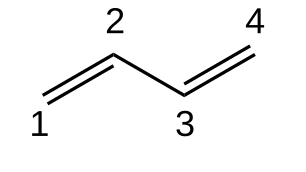
\includegraphics[scale=1.0]{./structures/exercise_1/trans-1,3-butadiene/0.png}
		\setlength{\abovecaptionskip}{-0.3em}
		\captionof{figure}{The order of carbon atoms in {\it trans}-1,3-butadiene.}
		\setlength{\belowcaptionskip}{-0.8em}
		\end{center}				

		For $\pi$-electron atomic orbitals' representation $\Gamma^{\rm AO}$, its following characters is listed below.
		\begin{center}
		\setlength{\abovecaptionskip}{-0.3em}
		\captionof{table}{The character of the $\pi$-electron atomic orbitals' representation $\Gamma^{\rm AO}$.}
		\begin{tabular}{ccccc}\hline
	$\mathscr{C}_{\rm 2h}$ & $E$ & $C_2$ & $i$ & $\sigma_h$ \\ \hline
	$\chi^{\AO}(C_i)$	&	4	&	0	&	0	&	-4	\\ \hline
		\end{tabular}\vspace*{-0.5em}
		\end{center}
		
		Relevant reduction coefficients are
		\begin{align*}
		a_g &= \frac{1}{4} \sum_{R} \chi^{\AO}(R) \chi^{A_g}(R) = \frac{1}{4} \left[ 1 \times 4 \times 1 + 1 \times 0 \times 1 + 1 \times 0 \times 1 + 1 \times (-4) \times 1 \right] = 0, \\
		b_g &= \frac{1}{4} \sum_{R} \chi^{\AO}(R) \chi^{B_g}(R) = \frac{1}{4} \left[ 1 \times 4 \times 1 + 1 \times 0 \times (-1) + 1 \times 0 \times 1 + 1 \times (-4) \times (-1) \right] = 2, \\
		a_u &= \frac{1}{4} \sum_{R} \chi^{\AO}(R) \chi^{A_u}(R) = \frac{1}{4} \left[ 1 \times 4 \times 1 + 1 \times 0 \times 1 + 1 \times 0 \times (-1) + 1 \times (-4) \times (-1) \right] = 2, \\
		b_u &= \frac{1}{4} \sum_{R} \chi^{\AO}(R) \chi^{B_u}(R) = \frac{1}{4} \left[ 1 \times 4 \times 1 + 1 \times 0 \times (-1) + 1 \times 0 \times (-1) + 1 \times (-4) \times 1 \right] = 0.
		\end{align*}
		
		Thus, we arrive at
		\begin{equation*}
			\Gamma^{\AO} = 2 \Gamma^{B_g} \oplus 2 \Gamma^{A_u}.
		\end{equation*}
		We conclude that there are two basis functions in the irreducible representation $\Gamma^{B_g}$ and $\Gamma^{A_u}$, respectively. Thus, to describe the effect of $O_R$, two suitable $2 \orbp_z$ atomic orbitals $\phi_i$ is enough.
		
		Thirdly, we inspect the transformation of $\phi_i$ under $O_R$ for the {\it trans}-1,3-butadiene, whose information is recorded below. We only list two $\phi_1$ and $\phi_2$, which is enough in current case.
		\begin{center}
		\setlength{\abovecaptionskip}{0em}
		\captionof{table}{Transformation of $\phi_i$ under $O_R$ for the {\it trans}-1,3-butadiene.}
		\begin{tabular}{ccccc}\hline
	$\mathscr{C}_{\rm 2h}$ & $O_E$ & $O_{C_2}$ & $O_i$ & $O_{\sigma_h}$ \\ \hline
			$\phi_1$	&	$\phi_1$	&	$\phi_4$	&	$-\phi_4$	&	$-\phi_1$	\\
			$\phi_2$	&	$\phi_2$	&	$\phi_3$	&	$-\phi_3$	&	$-\phi_2$	\\	\hline
		\end{tabular}
		\setlength{\belowcaptionskip}{0.5em}
		\end{center}
		
		For the irreducible representation $\Gamma^{B_g}$,
		\begin{align*}
		P^{B_g}\phi_1 &= \sum_{R} \chi^{B_g}(R) O_R \phi_1 = (O_E - O_{C_2} + O_{i} - O_{\sigma_h})\phi_1 = 2(\phi_1-\phi_4) , \\
		P^{B_g}\phi_2 &= \sum_{R} \chi^{B_g}(R) O_R \phi_2 = (O_E - O_{C_2} + O_{i} - O_{\sigma_h})\phi_2 = 2(\phi_2-\phi_3) .
		\end{align*}
		It is easy to find that they are mutually orthogonal. They can be normalized to
		\begin{align*}
		\phi^\prime_1 &= \frac{1}{\sqrt{2}} (\phi_1-\phi_4) , \\
		\phi^\prime_2 &= \frac{1}{\sqrt{2}} (\phi_2-\phi_3) .
		\end{align*}
		
		Then, the effective Hamitonian matrix elements for $\pi$ electrons can be calculated,
		\begin{align*}
		\Hp_{11} &= \int_{\RRR} \frac{1}{\sqrt{2}}(\phi_1-\phi_4) \Heff \frac{1}{\sqrt{2}}(\phi_1-\phi_4) = \frac{1}{2} (\alpha + 0 + 0 + \alpha) = \alpha, \\
		\Hp_{12} &= \int_{\RRR} \frac{1}{\sqrt{2}}(\phi_1-\phi_4) \Heff \frac{1}{\sqrt{2}}(\phi_2-\phi_3) = \frac{1}{2} (\beta - 0 - 0 + \beta) = \beta, \\
		\Hp_{22} &= \int_{\RRR} \frac{1}{\sqrt{2}}(\phi_2-\phi_3) \Heff \frac{1}{\sqrt{2}}(\phi_2-\phi_3) = \frac{1}{2} (\alpha - \beta - \beta + \alpha) = \alpha - \beta,
		\end{align*}
		viz.
		\begin{equation*}
			\Hp_{B_g} = \begin{pmatrix}
				\alpha	&	\beta \\ \beta & \alpha - \beta 
			\end{pmatrix}.
		\end{equation*}
		Next,
		\begin{align*}
			\det(\Hp_{B_g}-\varepsilon^\pi \Sp_{B_g}) = \begin{vmatrix}	
			\alpha-\varepsilon^\pi	&	\beta \\ 
			\beta & \alpha - \beta -\varepsilon^\pi	
\end{vmatrix} = \beta^2
\begin{vmatrix}
			x & 1 \\ 1 & x -1			
			\end{vmatrix} = \beta^2 ( x^x - x - 1 ) = 0,
		\end{align*}
		where
		\begin{equation*}
			x = \frac{\alpha-\varepsilon^\pi}{\beta}.
		\end{equation*}
		Current discriminant is
		\begin{equation*}
			\Delta_{B_g} = (-1)^2 - 4 \times 1 \times (-1) = 5,
		\end{equation*}				
		and then two roots are
		\begin{equation*}
			x_1 = \frac{1+\sqrt{5}}{2}, \quad x_2 = \frac{1-\sqrt{5}}{2},
		\end{equation*}
		which equal to	
		\begin{align}
			\varepsilon_1 &= \alpha - x_1 \beta = \alpha - \frac{1+\sqrt{5}}{2} \beta \approx \alpha - 1.618 \beta , \\
			\varepsilon_2 &= \alpha - x_2 \beta = \alpha - \frac{1-\sqrt{5}}{2} \beta = \alpha + \frac{\sqrt{5}-1}{2} \beta \approx \alpha + 0.618 \beta .
		\end{align}
		
		For $\Hp_{B_g}-\varepsilon^\pi_1 \Sp_{B_g}$, its reduced row echelon form is
		\begin{equation*}
			\begin{pmatrix}
				1	& \frac{-1+\sqrt{5}}{2}	\\	0	&	0
			\end{pmatrix},
		\end{equation*}
		which means
		\begin{equation*}
			\Phi_1 = -\frac{\sqrt{5}-1}{2}\phi^\prime_1 + \phi^\prime_2.
		\end{equation*}
		The sum of squares of coefficients is
		\begin{equation*}
			\sum_{i} c^2_i = (-\frac{\sqrt{5}-1}{2})^2 + 1^2 = \frac{5-\sqrt{5}}{2}.
		\end{equation*}
		
		Thus, we know
		\begin{align}
			\Phi^\pi_1 &= \sqrt{ \frac{2}{5-\sqrt{5}} } \Phi_1 = -\frac{\sqrt{5}-1}{2}\phi^\prime_1 + \phi^\prime_2 = - \sqrt{\frac{\sqrt{5}-1}{2\sqrt{5}}} \phi^\prime_1 + \sqrt{\frac{\sqrt{5}+1}{2\sqrt{5}}} \phi^\prime_2	\notag \\
			&= - \frac{1}{2}\sqrt{\frac{\sqrt{5}-1}{\sqrt{5}}}\phi_1  + \frac{1}{2}\sqrt{\frac{\sqrt{5}+1}{\sqrt{5}}} \phi_2 - \frac{1}{2}\sqrt{\frac{\sqrt{5}+1}{\sqrt{5}}} \phi_3 + \frac{1}{2}\sqrt{\frac{\sqrt{5}-1}{\sqrt{5}}} \phi_4 \notag \\
			&\approx -0.3717 \phi_1 + 0.6015 \phi_2 - 0.6015 \phi_3 + 0.3717 \phi_4.
		\end{align}
		
		Similarly, the reduced row echelon form of $\Hp_{B_g}-\varepsilon^\pi_2 \Sp_{B_g}$ is
		\begin{equation*}
			\begin{pmatrix}
				1	& \frac{-1-\sqrt{5}}{2}	\\	0	&	0
			\end{pmatrix},
		\end{equation*}		
		which means
		\begin{equation*}
			\Phi_2 = \frac{\sqrt{5}+1}{2}\phi^\prime_1 + \phi^\prime_2.
		\end{equation*}
		And then,
		\begin{align}
			\Phi^\pi_2 &= \sqrt{ \frac{2}{5+\sqrt{5}} } \Phi_2 = \frac{\sqrt{5}+1}{2}\phi^\prime_1 + \phi^\prime_2 = \sqrt{\frac{\sqrt{5}+1}{2\sqrt{5}}} \phi^\prime_1 + \sqrt{\frac{\sqrt{5}-1}{2\sqrt{5}}} \phi^\prime_2	\notag \\
			&= \frac{1}{2}\sqrt{\frac{\sqrt{5}+1}{\sqrt{5}}}\phi_1  + \frac{1}{2}\sqrt{\frac{\sqrt{5}-1}{\sqrt{5}}} \phi_2 - \frac{1}{2}\sqrt{\frac{\sqrt{5}-1}{\sqrt{5}}} \phi_3 - \frac{1}{2}\sqrt{\frac{\sqrt{5}+1}{\sqrt{5}}} \phi_4 \notag \\
			&\approx 0.6015\phi_1 + 0.3717 \phi_2 - 0.3717 \phi_3 -  0.6015\phi_4.
		\end{align}
		
		In conclusion, for the irreducible representation $\Gamma^{B_g}$, relevant results are listed below.
		
		\begin{center}
		\setlength{\abovecaptionskip}{-0.5em}
		\captionof{table}{The H{\"u}ckel MOs in the irreducible representation $\Gamma^{B_g}$ of {\it trans}-1,3-butadiene.}
		\begin{tabular}{ccc}\hline
		  order	&	eigenvalue		& 	eigenfunction	\\ \hline
			1	&$\alpha-1.618\beta$& 	$-0.3717 \phi_1 + 0.6015 \phi_2 - 0.6015 \phi_3 + 0.3717 \phi_4$ \\
			2	&$\alpha+0.618\beta$& 	$0.6015\phi_1 + 0.3717 \phi_2 - 0.3717 \phi_3 -  0.6015\phi_4$\\ \hline
		\end{tabular}
		\end{center}
		
		In the same way, for the irreducible representation $\Gamma^{A_u}$,
		\begin{align*}
		P^{A_u}\phi_1 &= \sum_{R} \chi^{A_u}(R) O_R \phi_1 = (O_E + O_{C_2} - O_{i} - O_{\sigma_h})\phi_1 = 2(\phi_1+\phi_4) , \\
		P^{A_u}\phi_2 &= \sum_{R} \chi^{A_u}(R) O_R \phi_2 = (O_E + O_{C_2} - O_{i} - O_{\sigma_h})\phi_2 = 2(\phi_2+\phi_3) .
		\end{align*}
		It is easy to find that they are mutually orthogonal, too. They can be normalized to
		\begin{align*}
		\phi^\prime_3 &= \frac{1}{\sqrt{2}} (\phi_1+\phi_4) , \\
		\phi^\prime_4 &= \frac{1}{\sqrt{2}} (\phi_2+\phi_3) .
		\end{align*}
		Then, the effective Hamiltonian can be constructed, viz.
		\begin{equation*}
			\Hp_{A_u} = \begin{pmatrix}
				\alpha	&	\beta \\ \beta & \alpha + \beta 
			\end{pmatrix}.
		\end{equation*}
		Next,
		\begin{align*}
			\det(\Hp_{A_u}-\varepsilon^\pi \Sp_{A_u}) = \begin{vmatrix}	
			\alpha-\varepsilon^\pi	&	\beta \\ 
			\beta & \alpha + \beta -\varepsilon^\pi	
\end{vmatrix} = \beta^2
\begin{vmatrix}
			x & 1 \\ 1 & x +1			
			\end{vmatrix} = \beta^2 ( x^x + x - 1 ) = 0.
		\end{align*}
		Current discriminant is
		\begin{equation*}
			\Delta_{A_u} = 1^2 - 4 \times 1 \times (-1) = 5,
		\end{equation*}		
		and then two roots are
		\begin{equation*}
			x_3 = \frac{-1+\sqrt{5}}{2}, \quad x_4 = \frac{-1-\sqrt{5}}{2},
		\end{equation*}
		which equal to
		\begin{align}
			\varepsilon_3 &= \alpha - x_3 \beta = \alpha - \frac{-1+\sqrt{5}}{2} \beta \approx \alpha - 0.618 \beta , \\
			\varepsilon_4 &= \alpha - x_4 \beta = \alpha - \frac{-1-\sqrt{5}}{2} \beta = \alpha + \frac{\sqrt{5}+1}{2} \beta \approx \alpha + 1.618 \beta .
		\end{align}
		
		For $\Hp_{A_u}-\varepsilon^\pi_3 \Sp_{A_u}$, its reduced row echelon form is
		\begin{equation*}
			\begin{pmatrix}
				1	& \frac{1+\sqrt{5}}{2}	\\	0	&	0
			\end{pmatrix},
		\end{equation*}		
		which means
		\begin{equation*}
			\Phi_3 = -\frac{\sqrt{5}+1}{2}\phi^\prime_3 + \phi^\prime_4.
		\end{equation*}
		Thus,
		\begin{align}
			\Phi^\pi_3 &= \sqrt{ \frac{2}{5+\sqrt{5}} } \Phi_3 = -\sqrt{\frac{\sqrt{5}+1}{2\sqrt{5}}} \phi^\prime_3 + \sqrt{\frac{\sqrt{5}-1}{2\sqrt{5}}} \phi^\prime_4 \notag	\\
			&= -\frac{1}{2}\sqrt{\frac{\sqrt{5}+1}{\sqrt{5}}}\phi_1  + \frac{1}{2}\sqrt{\frac{\sqrt{5}-1}{\sqrt{5}}} \phi_2 + \frac{1}{2}\sqrt{\frac{\sqrt{5}-1}{\sqrt{5}}} \phi_3 - \frac{1}{2}\sqrt{\frac{\sqrt{5}+1}{\sqrt{5}}} \phi_4 \notag \\
			&\approx -0.6015 \phi_1 + 0.3717 \phi_2 + 0.3717 \phi_3 - 0.6015 \phi_4.
		\end{align}
		
		For $\Hp_{A_u}-\varepsilon^\pi_4 \Sp_{A_u}$, its reduced row echelon form is
		\begin{equation*}
			\begin{pmatrix}
				1	& \frac{1-\sqrt{5}}{2}	\\	0	&	0
			\end{pmatrix},
		\end{equation*}		
		which means
		\begin{equation*}
			\Phi_4 = \frac{\sqrt{5}-1}{2}\phi^\prime_3 + \phi^\prime_4.
		\end{equation*}
		Thus,		
		\begin{align}
			\Phi^\pi_4 &= \sqrt{ \frac{2}{5-\sqrt{5}} } \Phi_4 = \sqrt{\frac{\sqrt{5}-1}{2\sqrt{5}}} \phi^\prime_3 + \sqrt{\frac{\sqrt{5}+1}{2\sqrt{5}}} \phi^\prime_4 \notag	\\
			&= \frac{1}{2}\sqrt{\frac{\sqrt{5}-1}{\sqrt{5}}}\phi_1  + \frac{1}{2}\sqrt{\frac{\sqrt{5}+1}{\sqrt{5}}} \phi_2 + \frac{1}{2}\sqrt{\frac{\sqrt{5}+1}{\sqrt{5}}} \phi_3 + \frac{1}{2}\sqrt{\frac{\sqrt{5}-1}{\sqrt{5}}} \phi_4 \notag \\
			&\approx 0.3717 \phi_1 + 0.6015 \phi_2 + 0.6015 \phi_3 + 0.3717 \phi_4.
		\end{align}
		
		In conclusion, for the irreducible representation $\Gamma^{A_u}$, relevant results are listed below.
		
		\begin{center}
		\setlength{\abovecaptionskip}{-0.5em}
		\captionof{table}{The H{\"u}ckel MOs in the irreducible representation $\Gamma^{A_u}$ of {\it trans}-1,3-butadiene.}
		\begin{tabular}{ccc}\hline
		  order	&	eigenvalue		& 	eigenfunction	\\ \hline
			1	&$\alpha-0.618\beta$& 	$-0.6015 \phi_1 + 0.3717 \phi_2 + 0.3717 \phi_3 - 0.6015 \phi_4$ \\
			2	&$\alpha+1.618\beta$& 	$0.3717\phi_1 + 0.6015 \phi_2 +0.6015 \phi_3 + 0.3717\phi_4$  \\	 \hline
		\end{tabular}
		\end{center}
		
		Now, we have obtained all results, which are shown as following.
		
		\begin{center}
		\setlength{\abovecaptionskip}{-0.5em}
		\captionof{table}{The H{\"u}ckel MOs in all irreducible representations of {\it trans}-1,3-butadiene.}
		\begin{tabular}{ccccccc}\hline
		order 	& orbital energy & irrep & $c_1$ & $c_2$ & $c_3$ &$c_4$ \\ \hline
			1	&	$\alpha+1.618\beta$	&	$A_u$	&	0.3717	&	0.6015	&	0.6015	&	0.3717	\\
			2	&	$\alpha+0.618\beta$	&	$B_g$	&	0.6015	&	0.3717	&	-0.3717	&	-0.6015	\\
			3	&	$\alpha-0.618\beta$	&	$A_u$	&	0.6015	&	-0.3717	&	-0.3717	&	0.6015	\\
			4	&	$\alpha-1.618\beta$	&	$B_g$	&	0.3717	&	-0.6015	&	0.6015	&	-0.3717	\\ \hline
		\end{tabular}
		\end{center}
		
		Besides, their phase diagrams have been painted in \Figref{fig:phase_diagram_1}. They obey the rule that the less nodal planes are, the lower orbital energy is.
		
		\begin{center}
		\begin{tabular}{cccc}
			\begin{minipage}[t]{0.22\linewidth}
			\centering
			\setlength{\abovecaptionskip}{0.5em}
			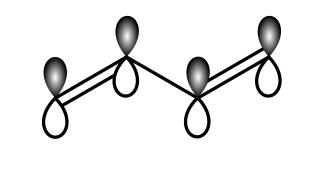
\includegraphics[scale=0.95]{./structures/exercise_1/trans-1,3-butadiene/4.png}
			\captionof*{figure}{$\varepsilon = \alpha + 1.618\beta$}
			\end{minipage} & 
			\begin{minipage}[t]{0.18\linewidth}
			\setlength{\abovecaptionskip}{0.5em}
			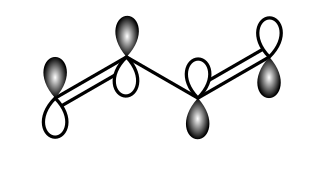
\includegraphics[scale=0.95]{./structures/exercise_1/trans-1,3-butadiene/2.png}
			\captionof*{figure}{$\varepsilon = \alpha + 0.618\beta$}
			\end{minipage} &
			\begin{minipage}[t]{0.22\linewidth}
			\centering
			\setlength{\abovecaptionskip}{0.5em}
			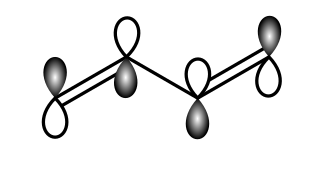
\includegraphics[scale=0.95]{./structures/exercise_1/trans-1,3-butadiene/3.png}
			\captionof*{figure}{$\varepsilon = \alpha - 0.618\beta$}
			\end{minipage} & 
			\begin{minipage}[t]{0.18\linewidth}
			\setlength{\abovecaptionskip}{0.5em}
			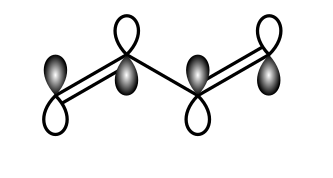
\includegraphics[scale=0.95]{./structures/exercise_1/trans-1,3-butadiene/1.png}
			\captionof*{figure}{$\varepsilon = \alpha - 1.618\beta$}
			\end{minipage}
		\end{tabular}				
		\captionof{figure}{Phase diagrams of these H{\"u}ckel MOs of {\it trans}-1,3-butadiene. Black bubbles mean plus phase while white ones mean minus phase. The color is used just for determining relative phase.}\label{fig:phase_diagram_1}
		\end{center}
		
		In the end, we conclude that for {\it trans}-1,3-butadiene, its ground state $\pi$-electron configuration is $(a_u)^2(b_g)^2$ and its delocalization energy is $2\times(1.618\beta+0.618\beta)-4\beta=0.472\beta$.